\begin{figure}[ht]
  \centering
  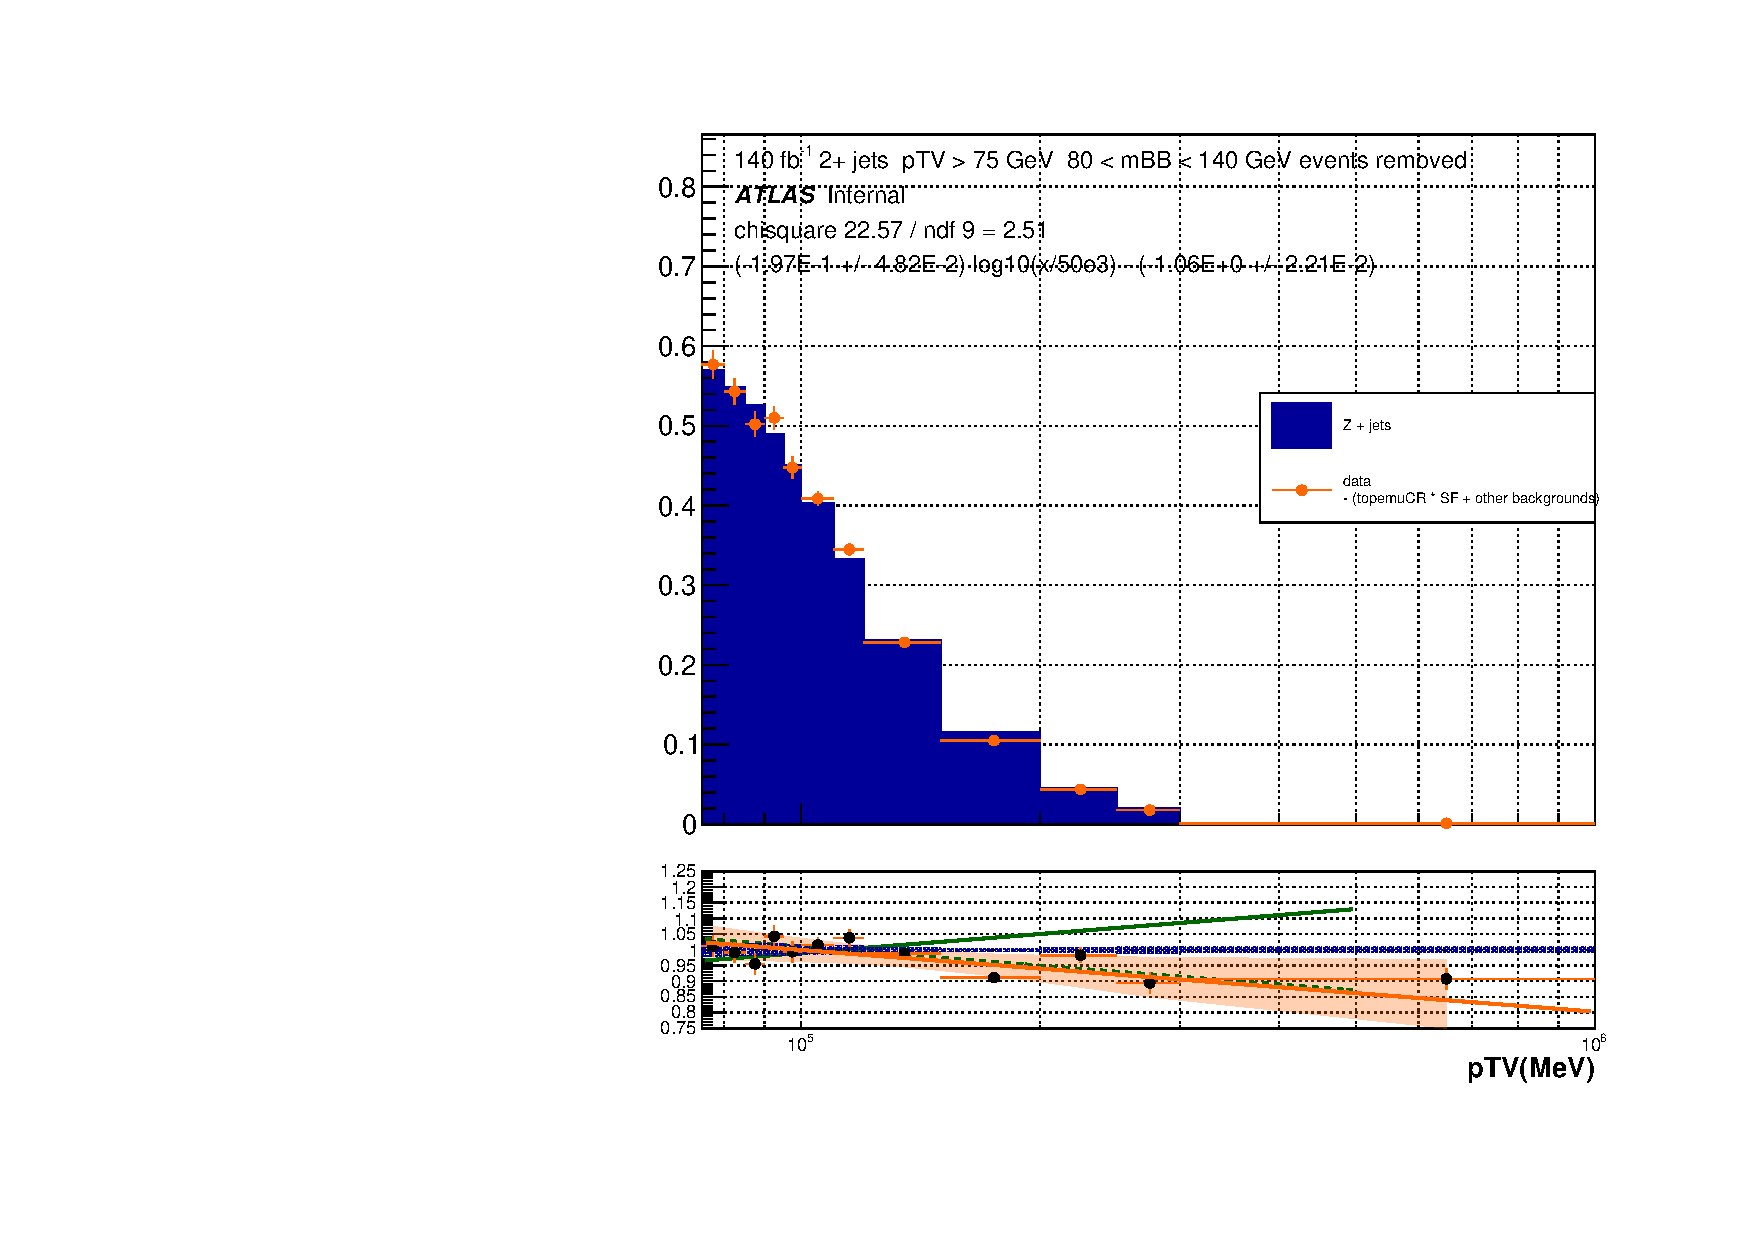
\includegraphics[width=0.59\textwidth]{Zjets-shapes/two_plus_jet_inclusive_blind_ttbardd/two_plus_jet_inclusive_blind_ttbardd_pTV_logx.pdf}
  \\
  \vspace{-8mm}
  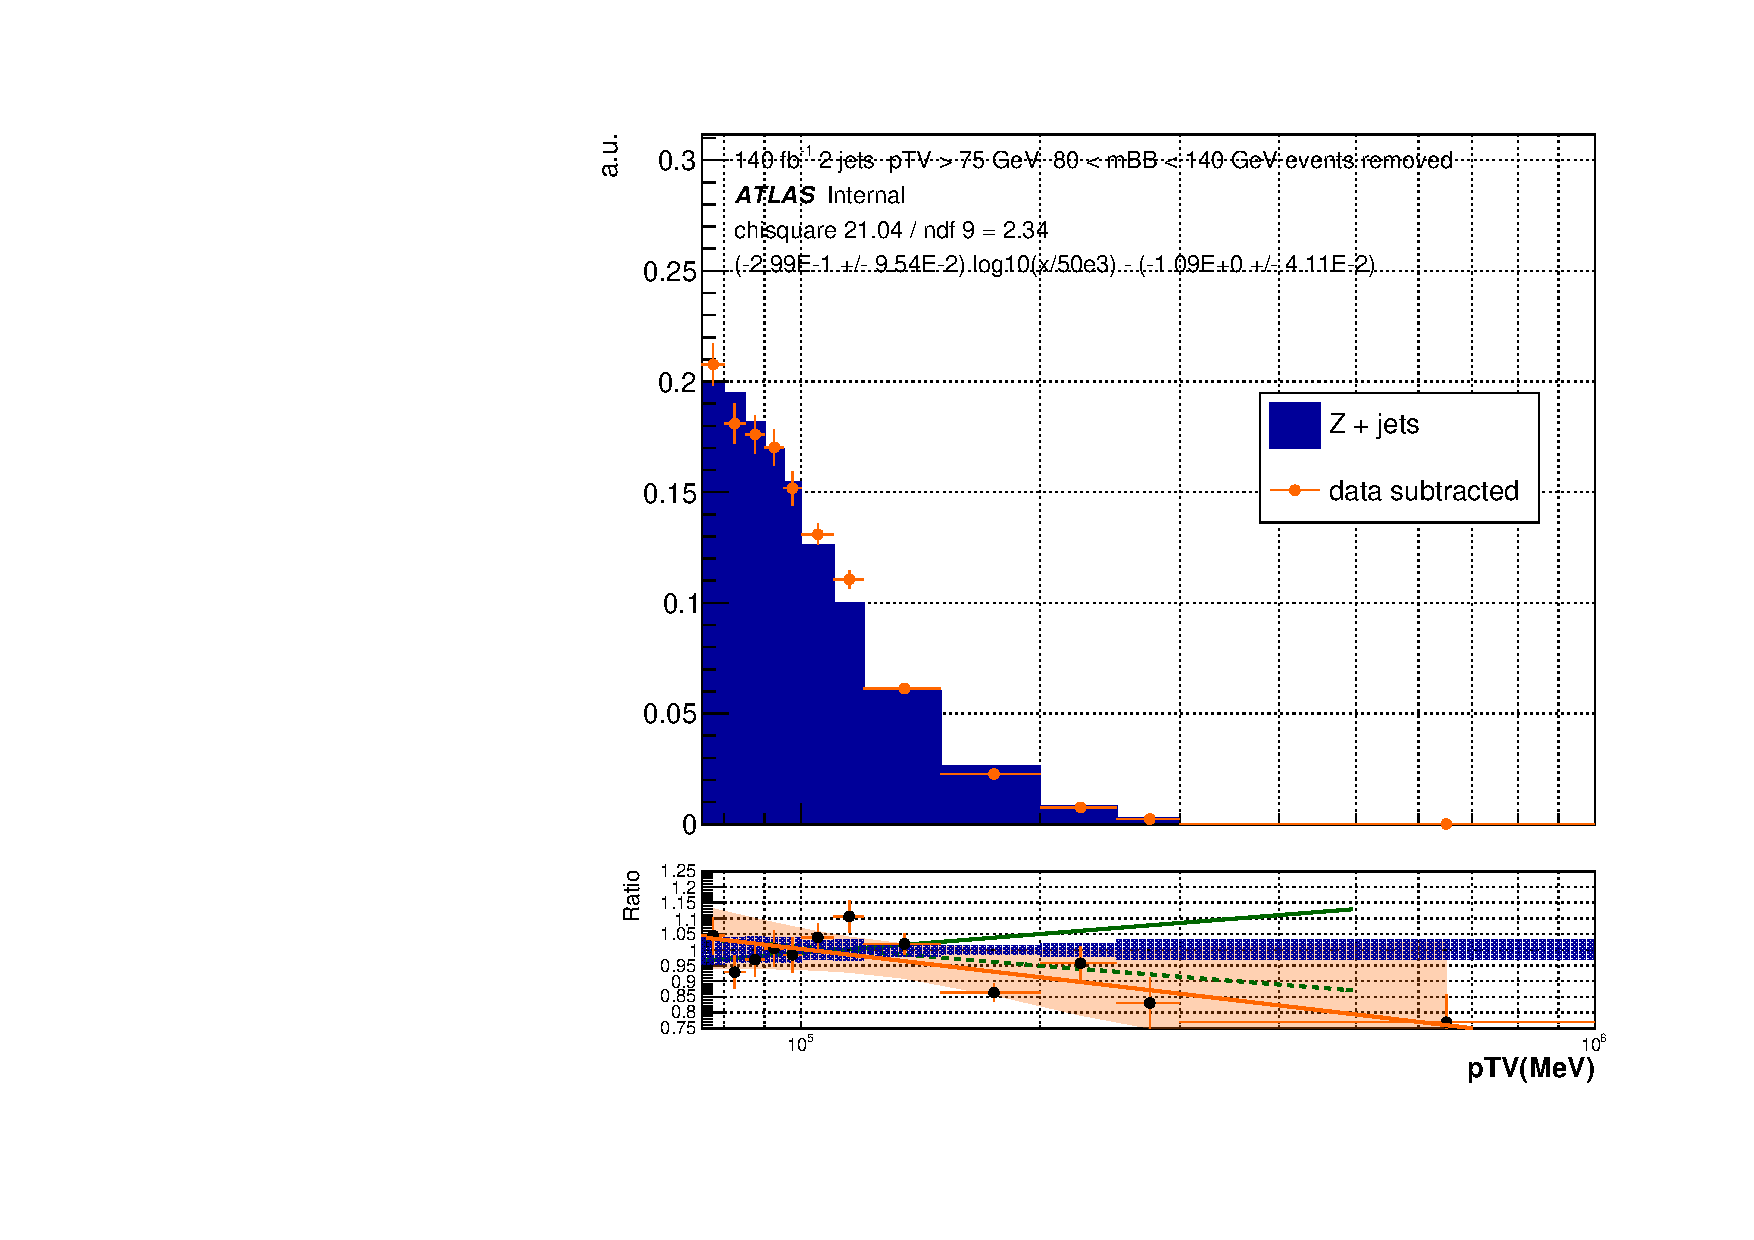
\includegraphics[width=0.59\textwidth]{Zjets-shapes/two_jet_inclusive_blind_ttbardd/two_jet_inclusive_blind_ttbardd_pTV_logx.pdf}
  \\
  \vspace{-8mm}
  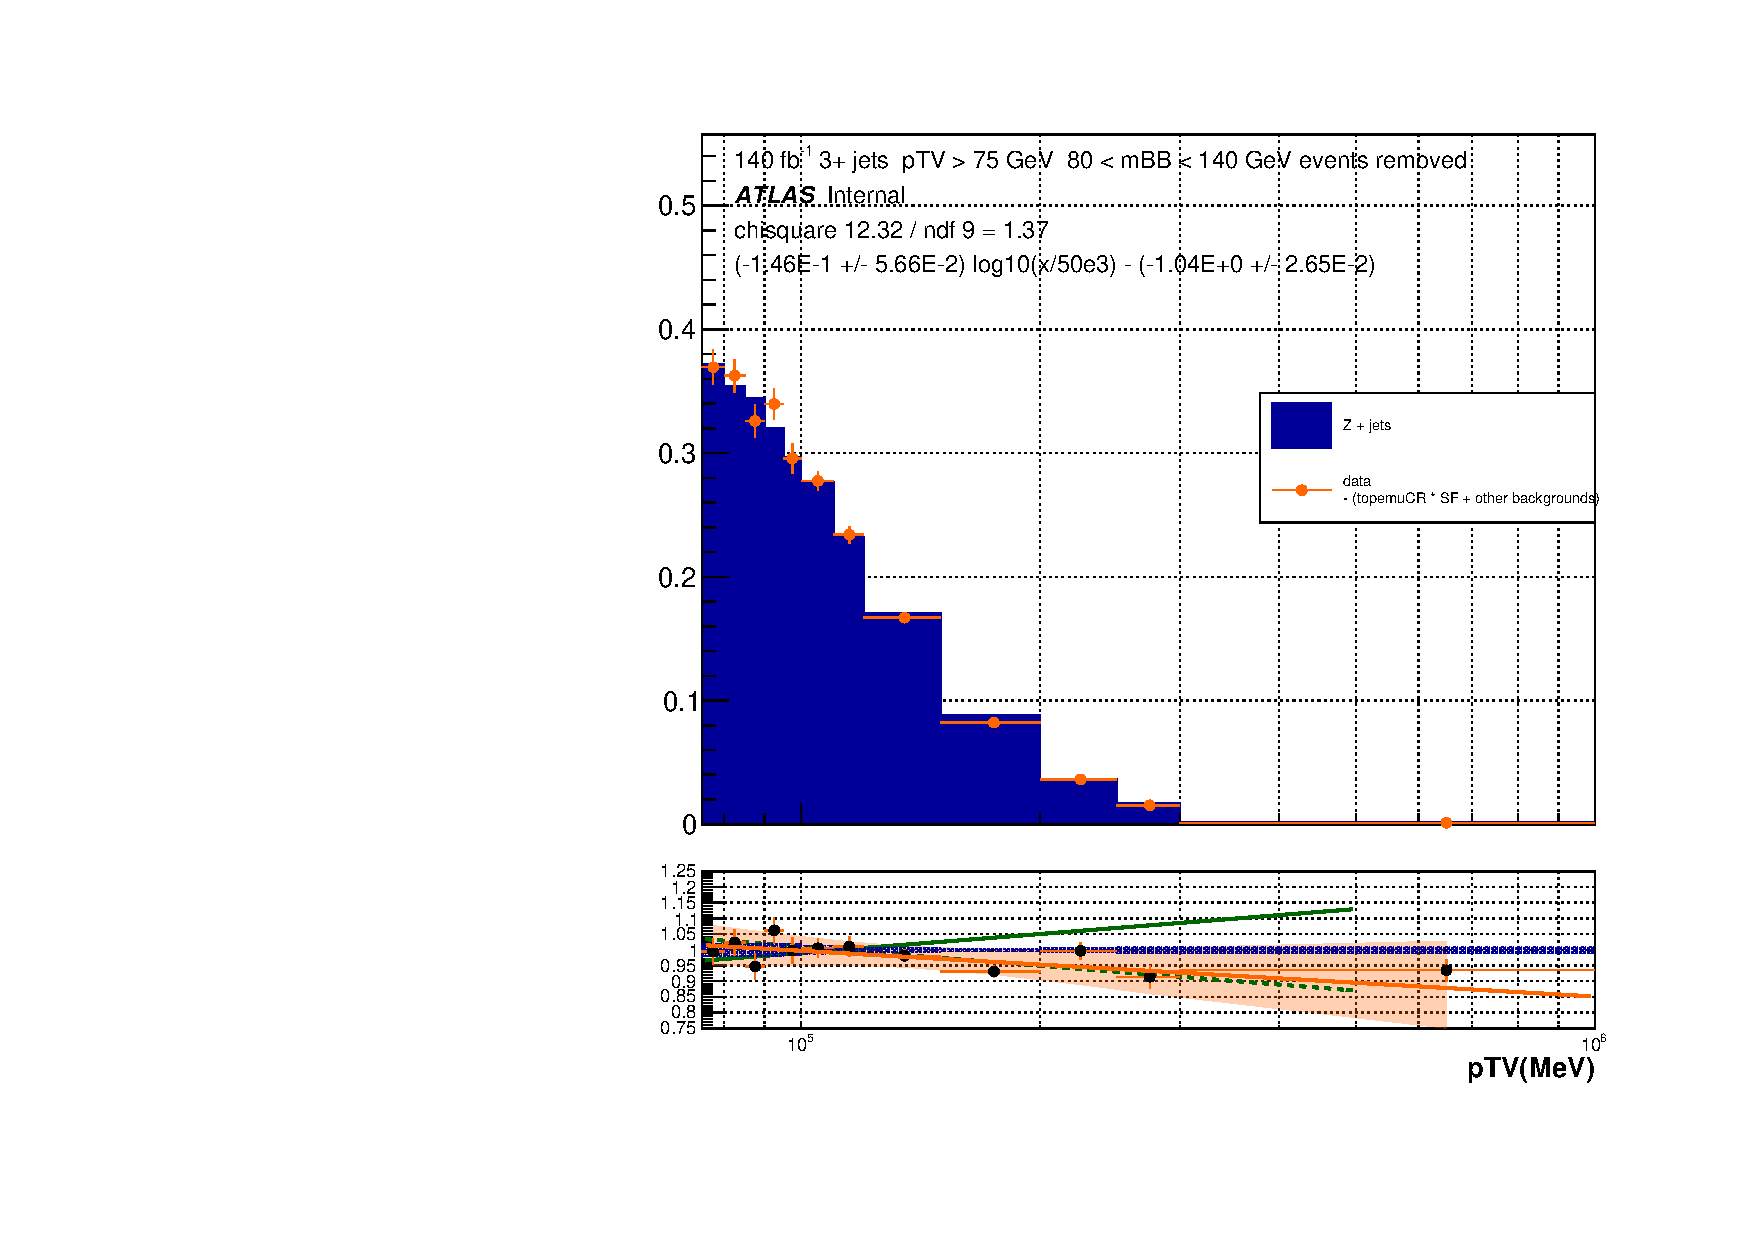
\includegraphics[width=0.59\textwidth]{Zjets-shapes/three_plus_jet_inclusive_blind_ttbardd/three_plus_jet_inclusive_blind_ttbardd_pTV_logx.pdf}
  \caption[Subtracted data versus the nominal $Z+$jets prediction,
  $p_{\mathrm{T}}^V$.]{\footnotesize Subtracted data versus the nominal $Z+$jets prediction
    in the $p_{\mathrm{T}}^V$ distribution. The green lines in the ratio show symmetrised
    uncertainty used in the previous analysis. The orange line is the fit to the
    ratio of the subtracted data and the prediction, the shaded region represents
    the 95~\% confidence interval.}
  \label{fig:zjets-ptv-shapes}
\end{figure}